\problemname{Dalarna}

\illustration{0.3}{dalarna.png}
\noindent
Harry loves Dalarna and dreams of making it Sweden's top-ranked county. 
After thorough analysis, he has determined that if every city $i$ in Dalarna had $p_i$ more car trips passing through, 
Dalarna would secure first place. To achieve this, Harry plans to order taxis to drive between the cities, 
with each taxi traveling along the shortest path between two cities.

Dalarna's road network consists of $N$ cities and $N-1$ roads. Each road directly connects two cities. 
If a taxi is in a city, it can travel to all cities that are directly connected to it via a road. Furthermore, 
the network is constructed so that it is always possible to travel between any pair of cities using one or more roads.

For each city $i$, Harry needs to ensure that at least $p_i$ taxis pass through the city to meet his goal. 
A taxi travels between two specified cities in the network and follows the shortest path.

To avoid raising suspicion, Harry wants to use as few taxis as possible. 
Help him calculate the minimum number of taxis he needs to order to meet the requirements.

\section*{Input}
The first line contains an integer $N$ ($1 \leq N \leq 10^5$), the number of cities in Dalarna.

The second line contains $N$ integers $p_1, p_2, ..., p_N$ ($0 \leq p_i \leq 10^9$), where $p_i$
indicates the number of taxis that must pass through city $i$.

The next $N-1$ lines describe the roads between the cities. Each line contains two integers $u$ and $v$
($1 \leq u, v \leq N$), indicating that there is a road between city $u$ and city $v$.
The road network connects all cities.

\section*{Output}
Print a single integer: the minimum number of taxis Harry needs to order.

\section*{Scoring}
Your solution will be tested on a set of test groups, each worth a number of points. Each test group contains
a set of test cases. To get the points for a test group you need to solve all test cases in the test group.

\noindent
\begin{tabular}{| l | l | p{12cm} |}
  \hline
  \textbf{Group} & \textbf{Points} & \textbf{Constraints} \\ \hline
  $1$    & $8$        & Each city is connected to at most 2 roads. \\ \hline
  $2$    & $11$       & $p_i = 1$ for all $i$. \\ \hline
  $3$    & $9$        & $p_i \leq 1$ for all $i$. \\ \hline
  $4$    & $12$       & $N \leq 7$, $p_i \leq 5$ for all $i$. \\ \hline
  $5$    & $14$       & $N \leq 100$, $p_i \leq 100$ for all $i$. \\ \hline
  $6$    & $15$       & $N \leq 1000$ \\ \hline
  $7$    & $31$       & No additional constraints. \\ \hline
\end{tabular}

\begin{figure}[h!]
  \centering
  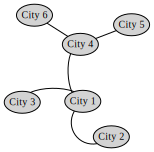
\includegraphics[width=0.3\textwidth]{dalarna_sample3.pdf}
  \caption{The road network for the 6 cities in sample 3.}
  \label{fig:dalarna_sample3}
\end{figure}

\begin{figure}[h!]
  \centering
  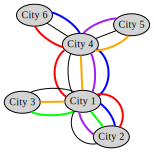
\includegraphics[width=0.3\textwidth]{dalarna_sample3b.pdf}
  \caption{A possible solution for sample 3, where the blue, orange, purple, green, and red paths represent 5 different taxi routes.}
  \label{fig:dalarna_sample3b}
\end{figure}
